\documentclass[tikz, a4paper]{nmd/hw}
\begin{document}
\classtemplate{SnapPy worksheet}{CURVES 2015}{\hfill}

\textbf{SnapPy website.} You can download SnapPy from
\url{http://snappy.computop.org}; the documentation contained there
can also be found on the Help menu in SnapPy itself. 

\textbf{The math behind SnapPy.}  See the excellent paper: J. Weeks, \emph{Computation of Hyperbolic Structures in Knot Theory}, \href{http://arxiv.org/abs/math/0309407}{arXiv:0309407}

\begin{problems}
  \item 
    \begin{enumerate}
      \item Load the manifold $v1234$ and name it $V$.  
      \item Use the browser to find the volume, Dirichlet domain, and
        symmetry group of $V$.
      \item Like any manifold in SnapPy, the object $V$ is really a
        particular \emph{triangulation} of this hyperbolic manifold.
        Back at the command line, determine the number of tetrahedra
        in the triangulation $V$.  Hint: Use tab completion by
        typing \texttt{V.<tab-key>}.  
      \item The manifold $V$ has one cusp.  Back the browser, do Dehn
        filling along the meridian curve.  What closed manifold do you get?  
    \end{enumerate}
 
\item 
  \begin{minipage}[t]{8.5cm}
  \begin{enumerate}
    \item Use SnapPy to find the name in the Rolfsen table for the link shown at
      right. 
    \item Is the projection at right the same as the one that's stored
      in SnapPy?  
    \end{enumerate}
  \end{minipage}\quad
  \begin{minipage}[t]{12cm}
    \hbox{}
    \vspace{-1cm}
    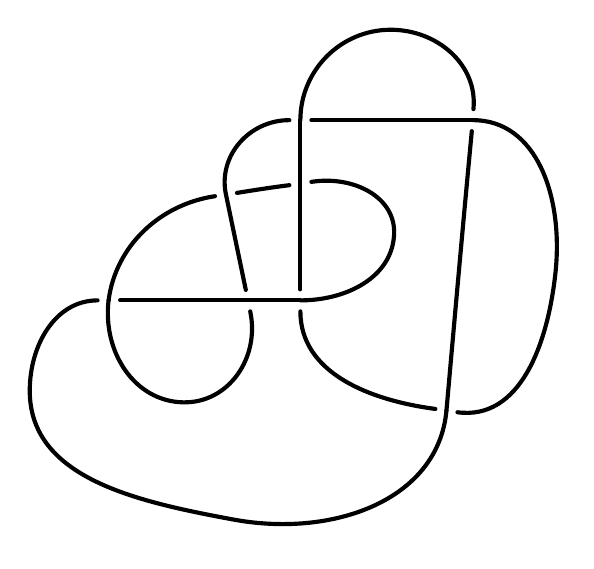
\begin{tikzpicture}[scale=0.7, line width=1.5, line cap=round, line join=round]
      \begin{scope}[color=black]
        \draw (7.49, 2.49) .. controls (6.28, 2.65) and (5.04, 3.15) .. (5.04, 4.26);
        \draw (5.04, 4.66) .. controls (5.04, 5.30) and (5.04, 5.94) .. (5.04, 6.58);
        \draw (5.04, 6.58) .. controls (5.04, 6.97) and (5.04, 7.35) .. (5.04, 7.73);
        \draw (5.04, 7.73) .. controls (5.04, 8.63) and (5.77, 9.37) .. 
          (6.68, 9.37) .. controls (7.53, 9.37) and (8.26, 8.73) .. (8.18, 7.93);
        \draw (8.15, 7.53) .. controls (7.99, 5.84) and (7.84, 4.15) .. (7.69, 2.46);
        \draw (7.69, 2.46) .. controls (7.54, 0.83) and (5.62, 0.14) .. 
          (3.79, 0.49) .. controls (2.08, 0.81) and (0.13, 1.23) .. 
          (0.13, 2.82) .. controls (0.13, 3.66) and (0.60, 4.46) .. (1.36, 4.46);
        \draw (1.77, 4.46) .. controls (2.54, 4.46) and (3.31, 4.46) .. (4.09, 4.46);
        \draw (4.09, 4.46) .. controls (4.41, 4.46) and (4.72, 4.46) .. (5.04, 4.46);
        \draw (5.04, 4.46) .. controls (5.88, 4.46) and (6.70, 4.88) .. 
          (6.74, 5.65) .. controls (6.78, 6.33) and (6.01, 6.73) .. (5.24, 6.61);
       \draw (4.84, 6.55) .. controls (4.52, 6.51) and (4.20, 6.46) .. (3.89, 6.41);
       \draw (3.49, 6.35) .. controls (2.49, 6.20) and (1.69, 5.45) .. (1.56, 4.46);
       \draw (1.56, 4.46) .. controls (1.45, 3.52) and (2.03, 2.63) .. 
          (2.91, 2.61) .. controls (3.73, 2.59) and (4.31, 3.41) .. (4.13, 4.26);
       \draw (4.05, 4.65) .. controls (3.93, 5.23) and (3.81, 5.80) .. (3.69, 6.38);
       \draw (3.69, 6.38) .. controls (3.54, 7.08) and (4.11, 7.73) .. (4.84, 7.73);
       \draw (5.24, 7.73) .. controls (6.22, 7.73) and (7.19, 7.73) .. (8.17, 7.73);
       \draw (8.17, 7.73) .. controls (9.33, 7.73) and (9.81, 6.34) .. 
          (9.67, 4.98) .. controls (9.53, 3.65) and (9.02, 2.28) .. (7.89, 2.43);
      \end{scope}
    \end{tikzpicture}
  \end{minipage}

\item In the morning session, I mostly focused on manifolds with
  cusps, but SnapPy also works with closed manifolds.  In particular,
  it comes with the Hodgson-Weeks census of small-volume closed
  hyperbolic 3-manifolds, which is called
  \texttt{OrientableClosedCensus}.

  \begin{enumerate}
    \item Use the ``?'' operator to find out more about
      \texttt{OrientableClosedCensus}; in particular, how many
      manifolds are in it?  

      Also, interrogate the orientable \emph{cusped} census to get
      ideas on how to select various types of manifolds for the later
      parts of this question.
      
    \item Closed manifold in SnapPy are represented as Dehn fillings
      on cusped manifolds.  You can do Dehn filling in the browser,
      via the \texttt{dehn\_fill} method, or as part of the
      specification that you given to \texttt{Manifold}.  For example,
      typing \texttt{A = Manifold(`4\_1(1,2)')} gives the closed
      3-manifold which is $\frac{1}{2}$-Dehn surgery on the figure 8
      knot.  Use the method \texttt{is\_isometric\_to} to show that
      $A$ is the sixth manifold the \texttt{OrientableClosedCensus}.
      Warning: In Python, lists are numbered starting from 0
      rather than 1.

    \item Find the unique manifold $M$ in the original
      \texttt{OrientableClosedCensus} whose volume is between $3.0$
      and $3.1$ and whose first homology is
      $\Z/3\Z \oplus \Z/3\Z \oplus \Z/3\Z$.

    \item Find a description of $M$ as Dehn surgery on a 3-component
      link in $S^3$.  Hint: Unfill the cusp in the default description
      of $M$ and then drill out the shortest geodesic twice.  

  \end{enumerate}

\item Here's how you get the exterior of a randomly chosen 14-crossing prime knot:

  \texttt{knots = HTLinkExteriors(cusps=1, crossings=14)} \\ 
  \texttt{M = knots.random()}

  \begin{enumerate}
    \item Python uses the \texttt{len} function to access the length of any
      list-like object, so do \texttt{len(knots)} to see how many such
      knots there are.

    \item Try creating the Dirichlet domain for $M$ at the command
      line.  Most of the time you will get an error message saying
      that this failed!  (If not, pick a different example which does
      fail for the rest of this problem ;-).

    \item By default, the hyperbolic structure on $M$ is computed
      using standard double-precision floating-point numbers (about 15
      decimal digits).  It turns out this isn't enough to find the
      Dirichlet domain for a manifold this complicated.  Use the
      \texttt{high\_precision} method of $M$ to upgrade it to a
      \texttt{ManifoldHP} called $H$. 

    \item Compute the volumes of $M$ and $H$.  Are the answers
      consistent with the hyperbolic structure on $H$ being computed
      to quad-double precision?

    \item Try computing the Dirichlet domain $D$ using $H$, which
      will most likely succeed though it typically takes a few
      seconds. 

    \item Interrogate $D$ to get a pretty picture and find out how
      many faces and vertices $D$ has. 

  \end{enumerate}

\end{problems}


\end{document}